% TODO famous example for a product line failure?

\subsection{Motivation}
\begin{frame}{Testing All Configurations}
	\begin{fancycolumns}
		\begin{exampletight}{}
			\centering\picDark[width=.75\textwidth]{productlines/featuremodels/db-constraint}
		\end{exampletight}
		
		\begin{example}{26 Valid Configurations}
			\footnotesize
			\leftandright{ % TODO transform to new template (deprecated) once nested fancycolumns work
				$\{B,G,W\}$\\
				$\{B,P,W\}$\\
				$\{B,G,P,W\}$\\
				$\{B,D,W\}$\\
				$\{B,G,D,W\}$\\
				$\{B,P,D,W\}$\\
				$\{B,G,P,D,W\}$\\
				$\{B,P,T,W\}$\\
				$\{B,G,P,T,W\}$\\
				$\{B,D,T,W\}$\\
				$\{B,G,D,T,W\}$\\
				$\{B,P,D,T,W\}$\\
				$\{B,G,P,D,T,W\}$
			}{
				$\{B,G,U\}$\\
				$\{B,P,U\}$\\
				$\{B,G,P,U\}$\\
				$\{B,D,U\}$\\
				$\{B,G,D,U\}$\\
				$\{B,P,D,U\}$\\
				$\{B,G,P,D,U\}$\\
				$\{B,P,T,U\}$\\
				$\{B,G,P,T,U\}$\\
				$\{B,D,T,U\}$\\
				$\{B,G,D,T,U\}$\\
				$\{B,P,D,T,U\}$\\
				$\{B,G,P,D,T,U\}$
			}
		\end{example}
		\nextcolumn
		\begin{note}{Discussion}
			\begin{itemize}
				\item only feasible for small product lines (few valid configurtions)
				\item redundant test effort
				\item large product lines: not even feasible to generate and compile all configurations
				\item (some) large product lines: not even the number of valid configurations is known
			\end{itemize}
		\end{note}
		% TODO add examples from Chico, diagram?
	\end{fancycolumns}
\end{frame}


\newcommand{\eemph}[1]{{\color{red}\textbf{#1}}}

\begin{frame}{Testing One Configuration}
	\begin{fancycolumns}
		\begin{exampletight}{}
			\centering\picDark[width=.75\textwidth]{productlines/featuremodels/db-constraint}
		\end{exampletight}
		
		\begin{example}{Which Valid Configuration to Test?}
			\footnotesize
			\leftandright{ % TODO tranform to new template (deprecated) once nested fancycolumns work
				$\{B,G,W\}$\\
				$\{B,P,W\}$\\
				$\{B,G,P,W\}$\\
				$\{B,D,W\}$\\
				$\{B,G,D,W\}$\\
				$\{B,P,D,W\}$\\
				$\{B,G,P,D,W\}$\\
				$\{B,P,T,W\}$\\
				$\{B,G,P,T,W\}$\\
				$\{B,D,T,W\}$\\
				$\{B,G,D,T,W\}$\\
				$\{B,P,D,T,W\}$\\
				\eemph{$\{B,G,P,D,T,W\}$}
			}{
				$\{B,G,U\}$\\
				$\{B,P,U\}$\\
				$\{B,G,P,U\}$\\
				$\{B,D,U\}$\\
				$\{B,G,D,U\}$\\
				$\{B,P,D,U\}$\\
				$\{B,G,P,D,U\}$\\
				$\{B,P,T,U\}$\\
				$\{B,G,P,T,U\}$\\
				$\{B,D,T,U\}$\\
				$\{B,G,D,T,U\}$\\
				$\{B,P,D,T,U\}$\\
				\emph{$\{B,G,P,D,T,U\}$}
			}
		\end{example}
		\nextcolumn
		\begin{note}{Discussion}
			\begin{itemize}
				\item applicable to large product lines
				\item no redundant test effort (from configurations)
				\item often not feasible to test all features in one configuration (e.g., Win and Unix)
				\item unnoticed feature interactions
			\end{itemize}
		\end{note}
		\begin{definition}{Feature Interactions} % TODO extra slide with an example
			\begin{itemize}
				\item features work well in isolation, but not in combination
				\item example: fire control and flood control in a building
				\item \emph{pairwise interactions}: interaction of two features
				\item \emph{t-wise interaction}: interaction of t features
			\end{itemize}
		\end{definition}
	\end{fancycolumns}
\end{frame}

\subsection{Pairwise Interaction Testing}
\begin{frame}{\insertsubsection}
	\begin{fancycolumns}
		\begin{definition}{Pairwise Interaction Testing}
			\begin{itemize}
				\item test a sample set $S \subseteq C$ of all valid configurations $C$ with pairwise coverage
				\item every pairwise interaction is covered by at least one configuration in the sample $S$
			\end{itemize}
		\end{definition}
		\begin{example}{Configurations with the Interaction Get $\wedge$ Put}
			\footnotesize
			\leftandright{ % TODO transform to new template (deprecated) once nested fancycolumns work
				$\{B,G,W\}$\\
				$\{B,P,W\}$\\
				\emph{$\{B,G,P,W\}$}\\
				$\{B,D,W\}$\\
				$\{B,G,D,W\}$\\
				$\{B,P,D,W\}$\\
				\eemph{$\{B,G,P,D,W\}$}\\
				$\{B,P,T,W\}$\\
				\eemph{$\{B,G,P,T,W\}$}\\
				$\{B,D,T,W\}$\\
				$\{B,G,D,T,W\}$\\
				$\{B,P,D,T,W\}$\\
				\eemph{$\{B,G,P,D,T,W\}$}
			}{
				$\{B,G,U\}$\\
				$\{B,P,U\}$\\
				\eemph{$\{B,G,P,U\}$}\\
				$\{B,D,U\}$\\
				$\{B,G,D,U\}$\\
				$\{B,P,D,U\}$\\
				\eemph{$\{B,G,P,D,U\}$}\\
				$\{B,P,T,U\}$\\
				\eemph{$\{B,G,P,T,U\}$}\\
				$\{B,D,T,U\}$\\
				$\{B,G,D,T,U\}$\\
				$\{B,P,D,T,U\}$\\
				\eemph{$\{B,G,P,D,T,U\}$}
			}
		\end{example}
		\nextcolumn
		\begin{note}{Discussion}
			\begin{itemize}
				\item applicable to large product lines
				\item reduced redundant effort compared to testing all configurations
				\item coverage guarantee (opposed to random configurations)
				\item still requires good test cases (program inputs)
				\item hard to compute small sample sets
			\end{itemize}
		\end{note}
		\begin{definition}{Pairwise Interactions}
			\begin{itemize}
				\item \emph{up-to} four interactions between $A$ and $B$
				\item both selected: $A \wedge B$
				\item one selected: $\neg A \wedge B$, $A \wedge \neg B$
				\item none selected: $\neg A \wedge \neg B$
			\end{itemize}
		\end{definition}
	\end{fancycolumns}
\end{frame}

\newcommand{\pair}[2]{$#1 \wedge #2$ & $#1 \wedge \neg #2$ & $\neg #1 \wedge #2$ & $\neg #1 \wedge \neg #2$\\}
\newcommand{\redandgray}[1]{\only<#1-| handout:#1->{\color{black}}\only<#1| handout:#1>{\color{blue}}}
\newcommand{\epair}[6]{
	{\redandgray{#3}$#1 \wedge #2$} & 
	{\redandgray{#4}$#1 \wedge \neg #2$} & 
	{\redandgray{#5}$\neg #1 \wedge #2$} & 
	{\redandgray{#6}$\neg #1 \wedge \neg #2$}\\
}
\newcommand{\clepair}[6]{
	{$#1 \wedge #2$} & 
	{$#1 \wedge \neg #2$} & 
	{$\neg #1 \wedge #2$} & 
	{$\neg #1 \wedge \neg #2$}\\
}

\begin{frame}{Pairwise Interaction Coverage}
	\begin{fancycolumns}[animation=none]
		\begin{definition}{Interactions to Cover}
			\begin{itemize}
				\item exclude invalid combinations (e.g., $W \wedge U$)
				\item exclude abstract features (e.g., $API$)
				\item exclude features contained in every configuration (e.g., $B$)
			\end{itemize}
		\end{definition}
		
		\begin{exampletight}{}
			\centering\picDark[width=\textwidth]{productlines/featuremodels/db-constraint}
		\end{exampletight}
		\nextcolumn
		\vspace{-10mm}
		\begin{example}{Pairwise Interactions}
			\centering\footnotesize\color{lightgray}
			\begin{tabular}{llll}
				\epair{G}{P}{3}{2}{1}{6}
				\epair{G}{D}{2}{3}{1}{5}
				\epair{G}{T}{3}{2}{1}{5}
				\epair{G}{W}{4}{2}{1}{6}
				\epair{G}{U}{2}{4}{6}{1}
				\epair{P}{D}{1}{3}{2}{4}
				\epair{P}{T}{1}{5}{6}{2}
				\epair{P}{W}{1}{3}{4}{2}
				\epair{P}{U}{3}{1}{2}{4}
				\epair{D}{T}{1}{2}{3}{4}
				\epair{D}{W}{1}{2}{4}{3}
				\epair{D}{U}{2}{1}{3}{4}
				\epair{T}{W}{1}{3}{4}{2}
				\epair{T}{U}{3}{1}{2}{4}
				& {\redandgray{1}$W \wedge \neg U$} & {\redandgray{2}$\neg W \wedge U$} & \\
			\end{tabular}
		\end{example}
		\begin{example}{Pairwise Coverage with Six Configurations}
			\footnotesize\color{lightgray}
			{\redandgray{1}$\{B,P,D,T,W\}$}\\
			{\redandgray{2}$\{B,G,D,U\}$}\\
			{\redandgray{3}$\{B,G,P,T,U\}$}\\
			{\redandgray{4}$\{B,G,W\}$}\\
			{\redandgray{5}$\{B,P,W\}$}\\
			{\redandgray{6}$\{B,D,T,U\}$}\\
		\end{example}
	\end{fancycolumns}
\end{frame}
% TODO use different colors for the different configurations (instead of separate handouts)

\subsection{T-Wise Interaction Testing}
\begin{frame}{\insertsubsection}
	\begin{fancycolumns}
		\begin{definition}{T-Wise Interaction Testing}
			\begin{itemize}
				\item generalization of pairwise interaction testing
				\item t-wise coverage: every t-wise interaction is covered by at least one configuration in the sample
				\item t=1: every feature is selected and also deselected
				\item t=2: pairwise interaction coverage
				\item t=3: every combination of three features
			\end{itemize}
		\end{definition}
		\begin{example}{{T=3 Interactions for the Features $G$, $P$, and $D$}}
			$G \wedge P \wedge D$ \hfill $G \wedge P \wedge \neg D$ \hfill $G \wedge \neg P \wedge D$
			
			$G \wedge \neg P \wedge \neg D$ \hfill $\neg G \wedge P \wedge D$ \hfill $\neg G \wedge P \wedge \neg D$
			
			$\neg G \wedge \neg P \wedge D$ \hfill $\neg G \wedge \neg P \wedge \neg D$
		\end{example}
		\nextcolumn
		\begin{exampletight}{Effectivity of Interaction Testing \mysource{\href{https://ieeexplore.ieee.org/document/1321063}{Kuhn et al.\ 2004}}}
			\footnotesize
			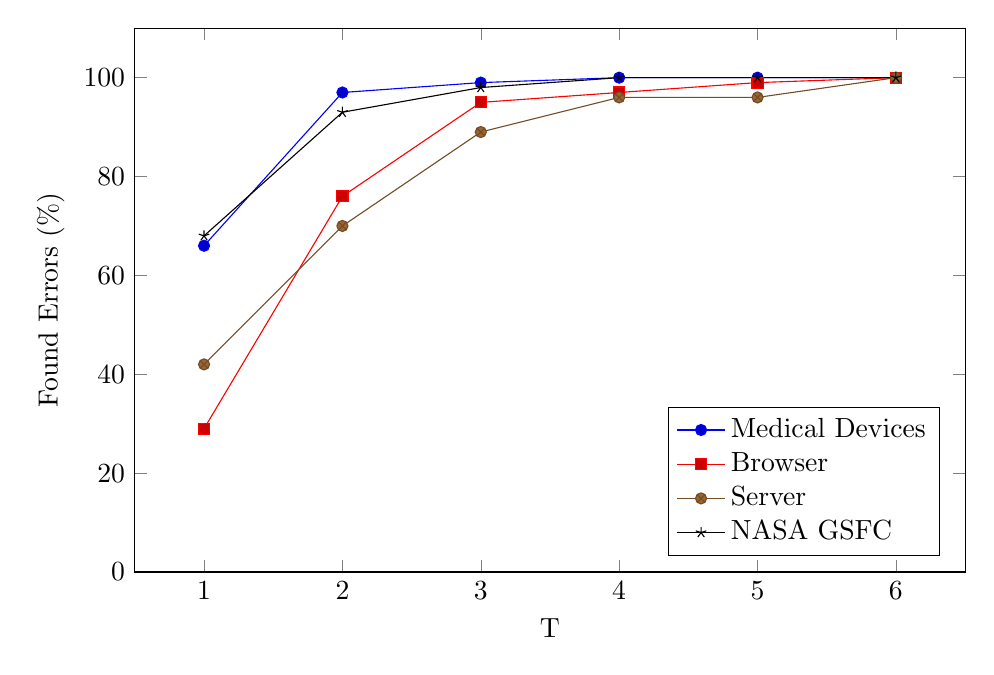
\begin{tikzpicture}
				\begin{axis}[
					width=\textwidth,height=.7\textwidth,
					%	ybar,
					ymin=0,ymax=110,
					xlabel=T,
					ylabel=Found Errors (\%),
					%	nodes near coords={\pgfmathprintnumber[precision=0]{\pgfplotspointmeta}},
					legend style={at={(0.97,0.03)},anchor=south east},
					legend cell align=left,
					]
					\addplot coordinates {(1,66) (2,97) (3,99) (4,100) (5,100) (6,100)};
					\addplot coordinates {(1,29) (2,76) (3,95) (4,97) (5,99) (6,100)};
					\addplot coordinates {(1,42) (2,70) (3,89) (4,96) (5,96) (6,100)};
					\addplot coordinates {(1,68) (2,93) (3,98) (4,100) (5,100) (6,100)};
					\legend{Medical Devices,Browser,Server,NASA GSFC}
				\end{axis}
			\end{tikzpicture}
		\end{exampletight}
		\begin{note}{Trade-Off}
			large t: high coverage (more effective)
			
			small t: low testing effort (more efficient)
		\end{note}
	\end{fancycolumns}
\end{frame}

\widexkcdframe{974} % salt 12s

%\begin{frame}{Einfache Heuristik für Pairwise Interaction Testing}
%	Greedy-Algorithmus: Wähle immer die Konfiguration als nächstes, die die meisten fehlenden Interaktionen abdeckt
%	\vspace{2mm}\pause
%	\begin{itemize}
	%		\item Erste Konfiguration frei wählbar (jede deckt am Anfang die gleiche Anzahl von Interaktionen ab: eine pro Paar)
	%		\item Stoppe wenn keine Interaktionen übrig
	%		\item Findet ggfs.\ nicht die kleinste Teilmenge an Konfigurationen
	%		\item Bessere Algorithmen wurden in den letzten Jahren vorgeschlagen (z.B. ICPL)
	%	\end{itemize}
%\end{frame}

% TODO introduce ICPL

\subsection{Combinatorial Interaction Testing in Practice}
\begin{frame}{Combinatorial Interaction Testing with ICPL\ \mytitlesource{\icpl}}
	\begin{fancycolumns}
		\begin{exampletight}{Assumption: All Features are Optional}
			\centering\pic[width=.66\textwidth]{productlines/optional-features}
		\end{exampletight}
		
		\begin{exampletight}{Number of Configurations in Pairwise Sample}
			\footnotesize\centering
			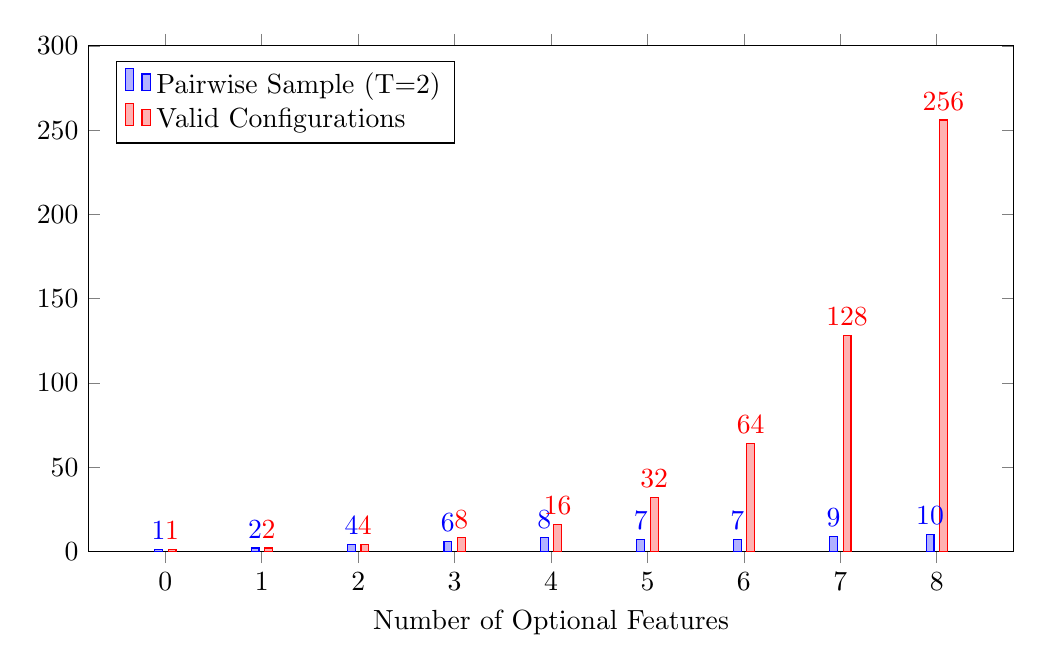
\begin{tikzpicture}
				\begin{axis}[
					width=1.1\textwidth,height=.66\textwidth,
					ybar,
					bar width=1mm,
					ymin=0,ymax=300,
					xlabel=Number of Optional Features,
					nodes near coords={\pgfmathprintnumber[precision=0]{\pgfplotspointmeta}},
					y label style={overlay},
					legend style={at={(0.03,0.97)},anchor=north west,fill=none},
					legend cell align=left,
					]
					\addplot coordinates {(0,1) (1,2) (2,4) (3,6) (4,8) (5,7) (6,7) (7,9) (8,10)};
					\addplot coordinates {(0,1) (1,2) (2,4) (3,8) (4,16) (5,32) (6,64) (7,128) (8,256)};
					\legend{Pairwise Sample (T=2),Valid Configurations}
				\end{axis}
			\end{tikzpicture}
		\end{exampletight}
		\nextcolumn
		\begin{exampletight}{Assumption: All Features are Optional}
			\centering\pic[width=.66\textwidth]{productlines/optional-features}
		\end{exampletight}
		
		\begin{exampletight}{Number of Configurations in T-Wise Sample}
			\footnotesize\centering
			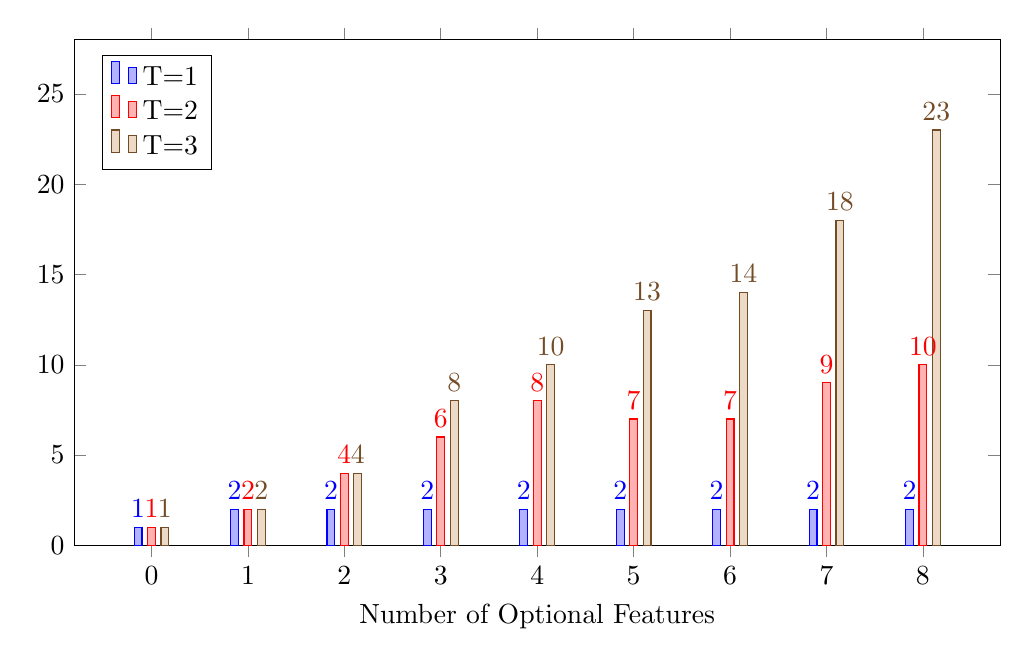
\begin{tikzpicture}
				\begin{axis}[
					width=1.1\textwidth,height=.66\textwidth,
					ybar,
					bar width=1mm,
					ymin=0,ymax=28,
					xlabel=Number of Optional Features,
					nodes near coords={\pgfmathprintnumber[precision=0]{\pgfplotspointmeta}},
					y label style={overlay},
					legend style={at={(0.03,0.97)},anchor=north west,fill=none},
					legend cell align=left,
					]
					\addplot coordinates {(0,1) (1,2) (2,2) (3,2) (4,2) (5,2) (6,2) (7,2) (8,2)};
					\addplot coordinates {(0,1) (1,2) (2,4) (3,6) (4,8) (5,7) (6,7) (7,9) (8,10)};
					\addplot coordinates {(0,1) (1,2) (2,4) (3,8) (4,10) (5,13) (6,14) (7,18) (8,23)};
					\legend{T=1,T=2,T=3}
				\end{axis}
			\end{tikzpicture}
		\end{exampletight}
	\end{fancycolumns}
\end{frame}

%\begin{frame}{Recap: Feature Model of the Linux Kernel}
%	\slideLinuxFeatureModel
%\end{frame}

\begin{frame}{Pairwise Interaction Testing in Practice\ \mytitlesource{\icpl}}
	\begin{fancycolumns}
		\begin{exampletight}{Time in Minutes to Compute Sample}
			\footnotesize\centering
			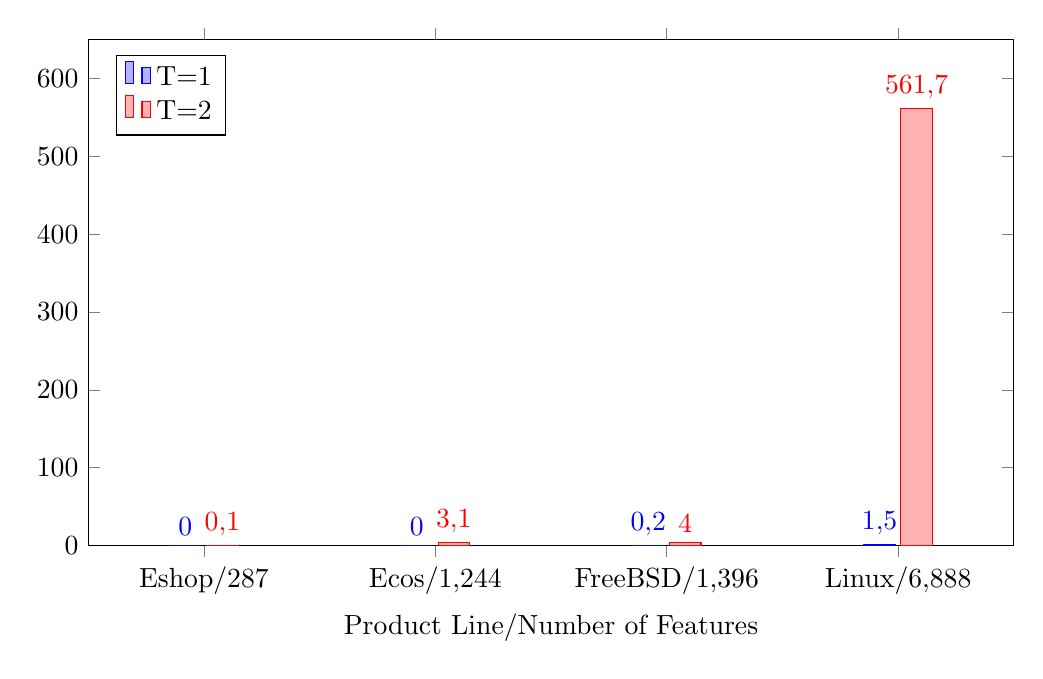
\begin{tikzpicture}
				\begin{axis}[
					/pgf/number format/.cd,use comma,1000 sep={.},
					width=1.1\textwidth,height=.66\textwidth,
					ybar,
					bar width=4mm,
					ymin=0,ymax=650,
					xmin=-.5,xmax=3.5,
					xlabel=Product Line/Number of Features,
					xtick={0,1,2,3},
					xticklabels={Eshop/287,{Ecos/1,244},{FreeBSD/1,396},{Linux/6,888}},
					nodes near coords={\pgfmathprintnumber[precision=1,fixed]{\pgfplotspointmeta}},
					y label style={overlay},
					legend style={at={(0.03,0.97)},anchor=north west,fill=none},
					legend cell align=left,
					]
					\addplot coordinates {(0,0) (1,0) (2,.2) (3,1.5)};
					\addplot coordinates {(0,.1) (1,3.1) (2,4.0) (3,561.7)};
					%	\addplot coordinates {(0,7.6) };
					\legend{T=1,T=2,T=3}
				\end{axis}
			\end{tikzpicture}
		\end{exampletight}
		\begin{example}{}
			\begin{itemize}
				\item about 9h for Linux
				\item 480 configuration in pairwise sample
			\end{itemize}
		\end{example}
		\nextcolumn
		\begin{exampletight}{Number of Configurations in Sample}
			\footnotesize\centering
			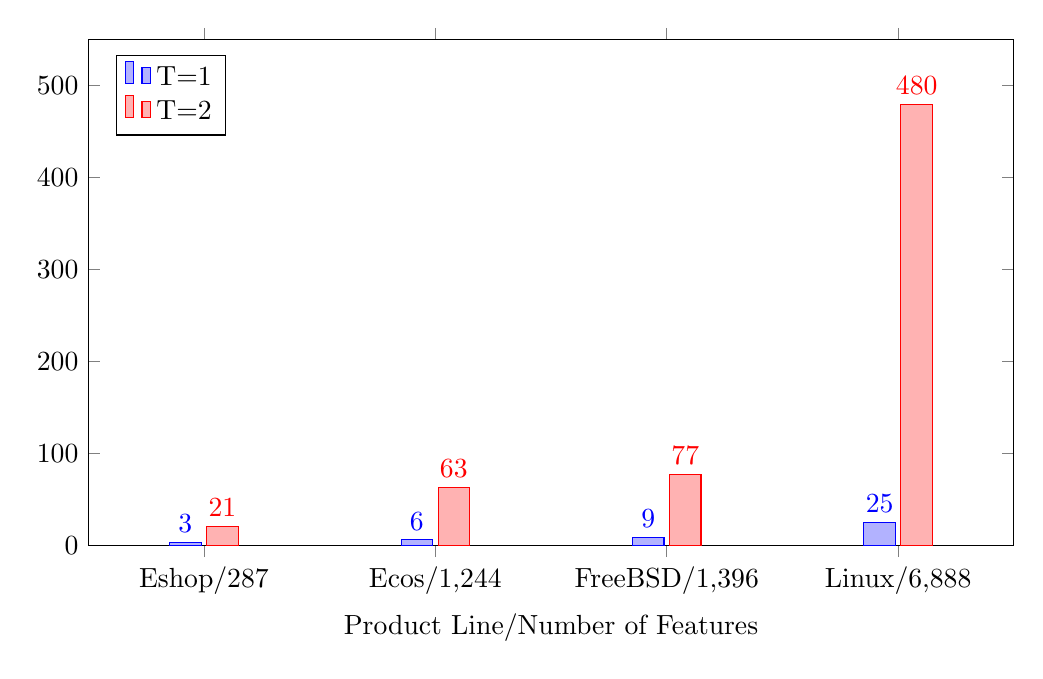
\begin{tikzpicture}
				\begin{axis}[
					/pgf/number format/.cd,use comma,1000 sep={.},
					width=1.1\textwidth,height=.66\textwidth,
					ybar,
					bar width=4mm,
					ymin=0,ymax=550,
					xmin=-.5,xmax=3.5,
					xlabel=Product Line/Number of Features,
					xtick={0,1,2,3},
					xticklabels={Eshop/287,{Ecos/1,244},{FreeBSD/1,396},{Linux/6,888}},
					nodes near coords={\pgfmathprintnumber[precision=0]{\pgfplotspointmeta}},
					y label style={overlay},
					legend style={at={(0.03,0.97)},anchor=north west,fill=none},
					legend cell align=left,
					]
					\addplot coordinates {(0,3) (1,6) (2,9) (3,25)};
					\addplot coordinates {(0,21) (1,63) (2,77) (3,480)};
					%	\addplot coordinates {(0,108) };
					\legend{T=1,T=2,T=3}
				\end{axis}
			\end{tikzpicture}
		\end{exampletight}
		\begin{example}{}
			\begin{itemize}
				\item Linux kernel v2.6.28.6 (February 2009)
				\item 6,888 features, 187,193 clauses in conjunctive normal form
			\end{itemize}
		\end{example}
	\end{fancycolumns}
\end{frame}

% TODO how Linux is developed: patches on mailing list, only considered if not rejected by CI, what happens in CI

% TODO variant reduction, prevent the explosion. marketing wants them all. engineering and quality assurance too expensive.

\begin{frame}{Number of Features in Linux\ \mytitlesource{\href{https://www4.cs.fau.de/Ausarbeitung/MA-I4-2015-04-Hengelein.pdf}{Hengelein 2015}}}
	\begin{fancycolumns}[widths={70}]
		\begin{exampletight}{{2005--2015: Number of Features Tripled}}
			\pic[width=\linewidth]{productlines/linux-features}
		\end{exampletight}
	\end{fancycolumns}
\end{frame}

\subsection{Wisdom on Features}
\begin{frame}{Choose Features Wisely}
	\begin{fancycolumns}
		\begin{exampletight}{John Ferguson Smart (2017)}
			\centering\picDark[width=.98\linewidth,angle=2,trim=0 0 5 0,clip]{productlines/unnecessary-features}
		\end{exampletight}
		% 
		\nextcolumn
		\centering\pic[width=.47\linewidth,trim=0 0 0 0,clip]{people/john-carmack}
		\vspace{-7mm}
		
		\begin{note}{John Carmack (born 1970) \mysource{\href{https://www.ics.uci.edu/~pattis/quotations.html\#C}{uci.edu}}}
			\mycite{The important point is that the cost of adding a feature isn't just the time it takes to code it. The cost also includes the addition of an obstacle to future expansion. %Sure, any given feature list can be implemented, given enough coding time. But in addition to coming out late, you will usually wind up with a codebase that is so fragile that new ideas that should be dead-simple wind up taking longer and longer to work into the tangled existing web. 
				[...] The trick is to pick the features that don't fight each other.}
		\end{note}
		% video game developer, co-founder of a video game company
	\end{fancycolumns}
\end{frame}
